A portion of the data contained in Table 6.10 in Chapter 6 is reproduced in Table 5.13.
These data represent various costs associated with transporting milk from farms to dairy
plants for gasoline trucks. Only the first 25 multivatiate observations for gasoline trucks
are given. Observations 9 and 21 have been identified as outliers from the full data set of
36 observations. (See [2].)

\begin{enumerate}[label= (\alph*)]
    \item Construct \textit{Q-Q} plots of the marginal distributions of fuel, repair, and capital costs.
    Also, construct the three possible scatter diagrams from the pairs of observations on
    different variables. Are the outliers evident? Repeat the \textit{Q-Q} plots and the scatter
    diagrams with the apparent outliers removed. Do the data now appear to be normally
    distributed? Discuss.

    \begin{figure}[H]
        \centering
        \begin{tabular}{cc}
            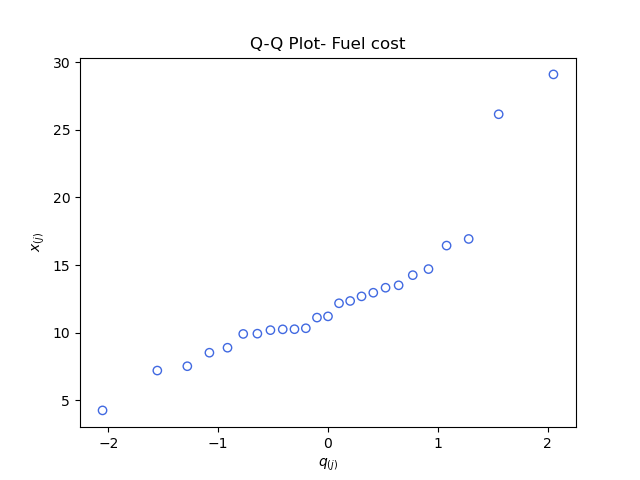
\includegraphics[scale=0.30]{./python/chapter-5/Question-5-22-a-QQ-Fuel.png} &
            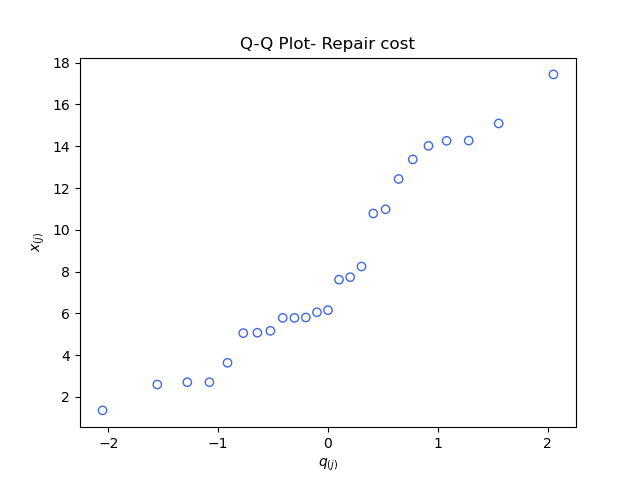
\includegraphics[scale=0.30]{./python/chapter-5/Question-5-22-a-QQ-Repair.png} \\
            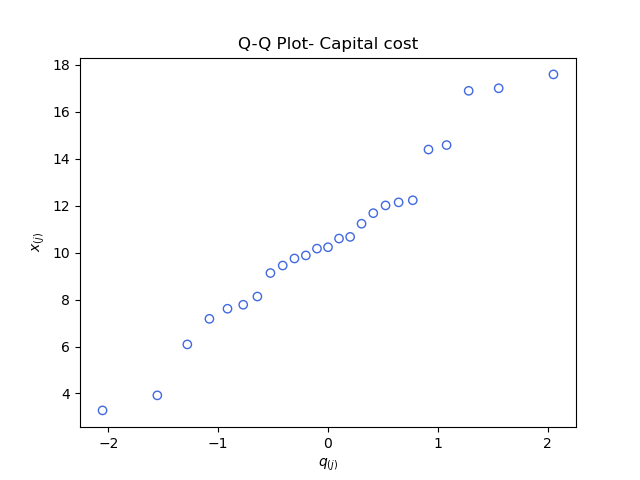
\includegraphics[scale=0.30]{./python/chapter-5/Question-5-22-a-QQ-Capital.png}
        \end{tabular}
    \end{figure}

    \begin{figure}[H]
        \centering
        \begin{tabular}{cc}
            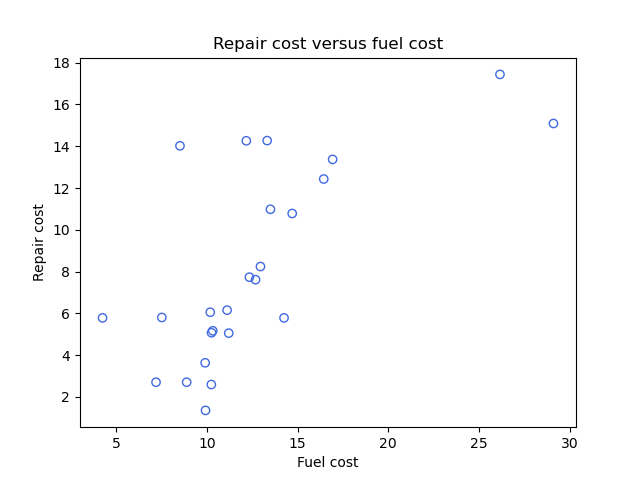
\includegraphics[scale=0.30]{./python/chapter-5/Question-5-22-a-xy-FuelRepair.png} &
            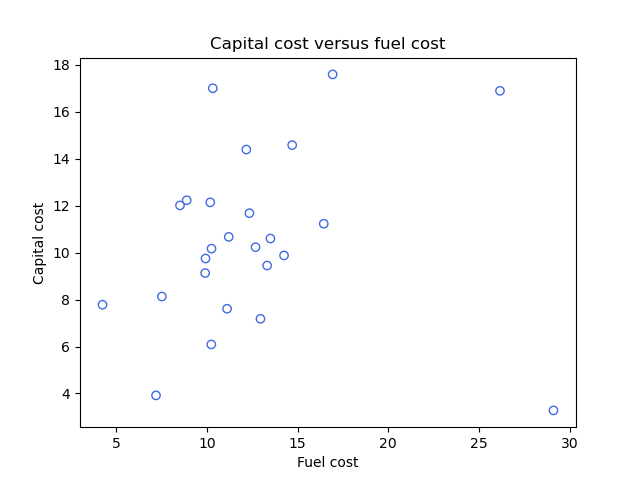
\includegraphics[scale=0.30]{./python/chapter-5/Question-5-22-a-xy-FuelCapital.png} \\
            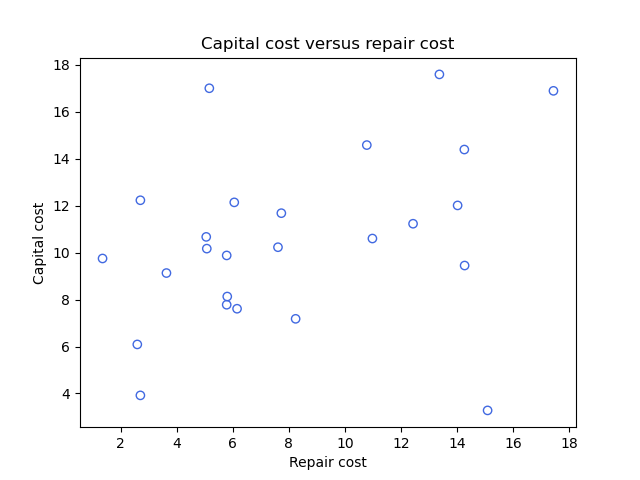
\includegraphics[scale=0.30]{./python/chapter-5/Question-5-22-a-xy-RepairCapital.png}
        \end{tabular}
    \end{figure}

    The \textit{Q-Q} plot for fuel looks the worst. There are two obvious outliers (observations 9 and 21) with higher values than the rest. The \textit{Q-Q} plot for repair look okay, but does have a hump in the upper portion of the plot. The \textit{Q-Q} plot for capital looks best, most linear, of the three. The bivariate scatterplots show the same two outliers of observations 9 and 21 from the fuel \textit{Q-Q} plot. None of the bivariate plots are obviously elliptical in shape, but we only have 25 observations.

    Removing the outlier observations, 9 and 21. Plots are below.

    \begin{figure}[H]
        \centering
        \begin{tabular}{cc}
            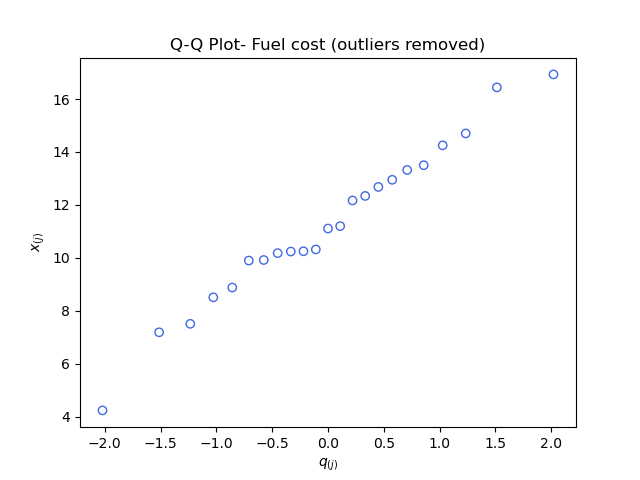
\includegraphics[scale=0.30]{./python/chapter-5/Question-5-22-a-QQ-Fuel-del.png} &
            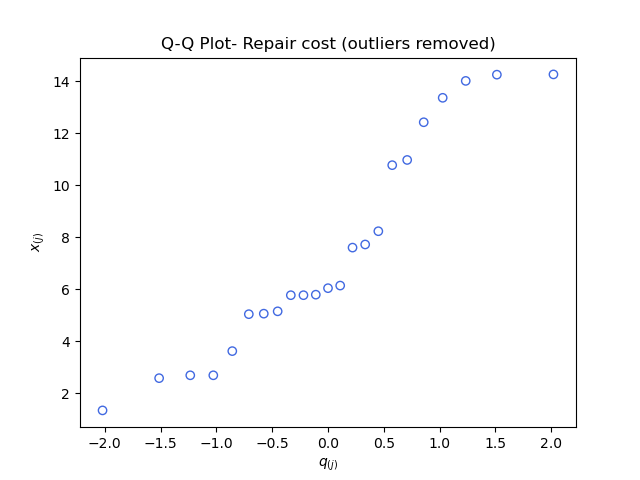
\includegraphics[scale=0.30]{./python/chapter-5/Question-5-22-a-QQ-Repair-del.png} \\
            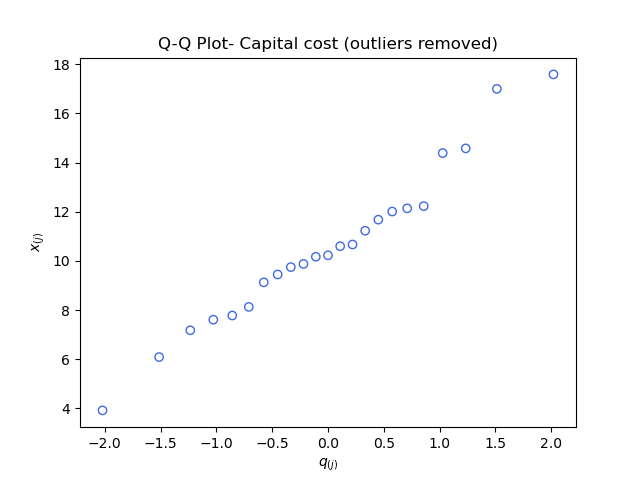
\includegraphics[scale=0.30]{./python/chapter-5/Question-5-22-a-QQ-Capital-del.png}
        \end{tabular}
    \end{figure}

    \begin{figure}[H]
        \centering
        \begin{tabular}{cc}
            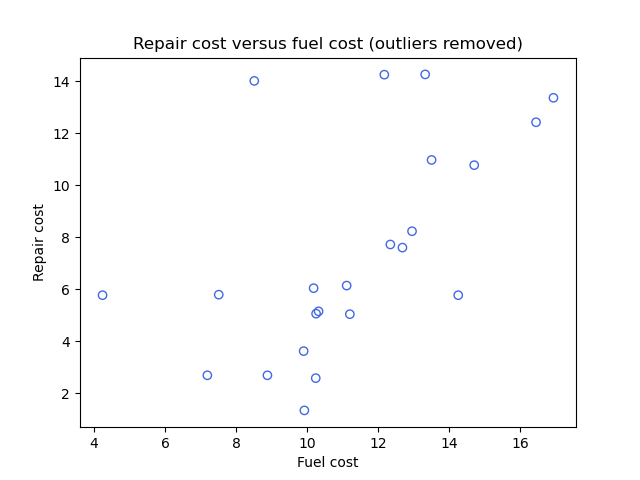
\includegraphics[scale=0.30]{./python/chapter-5/Question-5-22-a-xy-FuelRepair-del.png} &
            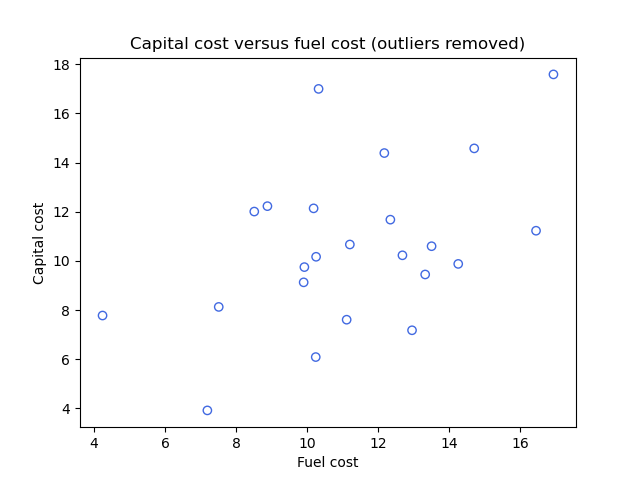
\includegraphics[scale=0.30]{./python/chapter-5/Question-5-22-a-xy-FuelCapital-del.png} \\
            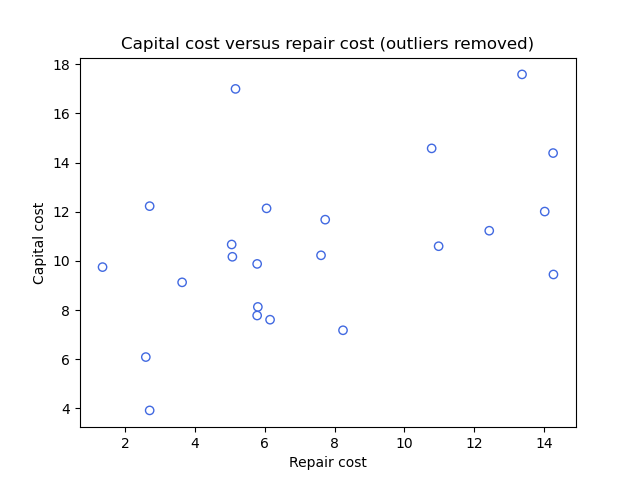
\includegraphics[scale=0.30]{./python/chapter-5/Question-5-22-a-xy-RepairCapital-del.png}
        \end{tabular}
    \end{figure}

    Removing the observations improved the \textit{Q-Q} plots for fuel and capital. The \textit{Q-Q} plot for repair, still has some curve in it. The scatterplots for our data still don't appear to be very elliptical, but we only have 23 observations, so maybe a visual determination isn't the best way to go about it.

    \item Construct 95\% Bonferroni intervals for the individual cost means. Also, find the 95\% $T^{2}$-intervals. Compare the two sets of intervals.
    
    \[
        \bar{\textbf{x}}
        =
        \begin{bNiceArray}{c}
            12.56 \\
            8.16 \\
            10.54
        \end{bNiceArray}
        \hspace{0.20cm}
        \text{and}
        \hspace{0.20cm}
        \begin{bNiceArray}{rrr}
            28.966 & 17.215 &  2.695 \\
            17.215 & 21.453 &  6.045 \\
             2.695 &  6.045 & 13.599
        \end{bNiceArray}
    \]
    The 95\% $T^{2}$ simultaneous confidence intervals:
    \[
    \bar{x}_{i}
    \pm
    \sqrt{
        \frac{(n-1)p}{(n-p)}
        F_{p, n-p}\left(\alpha\right)
    }
    \sqrt{
        \frac{s_{ii}}{n}
    }
    \]

    \[
        \begin{NiceArray}{rrrr}
        12.56 \pm \sqrt{9.98} \frac{\sqrt{28.97}}{\sqrt{25}} & \text{contains } \mu_{1} & \text{ or } & 9.16 \leq \mu_{1} \leq 15.96 \\
        8.16 \pm \sqrt{9.98} \frac{\sqrt{21.45}}{\sqrt{25}} & \text{contains } \mu_{2} & \text{ or } & 5.23 \leq \mu_{2} \leq 11.09 \\
        10.54 \pm \sqrt{9.98} \frac{\sqrt{13.60}}{\sqrt{25}} & \text{contains } \mu_{2} & \text{ or } & 8.21 \leq \mu_{3} \leq 12.87
        \end{NiceArray}
    \]
    The 95\% Bonferroni confidence intervals:
\[
    \bar{x}_{i}
    \pm
    t_{n-1}
    \left(\frac{\alpha}{2m}\right)
    \sqrt{
        \frac{
                s_{ii}
            }{
                n
            }
        }
\]

\[
    \begin{NiceArray}{rrrr}
       12.56 \pm 2.57 \frac{\sqrt{28.97}}{\sqrt{25}} & \text{contains } \mu_{1} & \text{ or } & 9.79 \leq \mu_{1} \leq 15.33 \\
       8.16 \pm 2.57 \frac{\sqrt{21.45}}{\sqrt{25}} & \text{contains } \mu_{2} & \text{ or } & 5.78 \leq \mu_{2} \leq 10.55 \\
       10.54 \pm 2.57 \frac{\sqrt{13.60}}{\sqrt{25}} & \text{contains } \mu_{2} & \text{ or } & 8.65 \leq \mu_{3} \leq 12.44
    \end{NiceArray}
\]

Dividing the length of the Bonferroni interval by the length of the $T^{2}$ interval,
\[
    \frac{\text{Length of Bonferroni interval}}{\text{Length of the }T^{2}\text{-interval}}
    =
    \frac{t_{n-1}(\frac{\alpha}{2m})}{\sqrt{\frac{(n-1)p}{n-p}F_{p, n-p}(\alpha)}}
    =
    0.8147
\]
The Bonferroni interval is only 81.47\% of the length of the simultaneous $T^{2}$ interval, so it's about 20\% shorter.

\end{enumerate}